\begin{Schunk}
\begin{Sinput}
> library("Ham94", lib.loc = "../../../library")
\end{Sinput}
\end{Schunk}
Pages 55 shows some realizations of AR processes.  We will assume the innovations are
drawn from a standard normal distribution.
\begin{Schunk}
\begin{Sinput}
> specifications <- list(list(label = "f = 0", MA = vector(mode = "numeric"), 
+     AR = vector(mode = "numeric")), list(label = "f = .5", MA = vector(mode = "numeric"), 
+     AR = c(0.5)), list(label = "f = .9", MA = vector(mode = "numeric"), 
+     AR = c(0.9)))
> T <- 100
> epsilon <- rnorm(T, 0, 1)
\end{Sinput}
\end{Schunk}
These can be calculated by iterating forward on the defining equations.
\begin{Schunk}
\begin{Sinput}
> simulate.forward <- function(specification, epsilon) {
+     T <- length(epsilon)
+     AR <- specification$AR
+     MA <- specification$MA
+     presample <- rep(0, max(length(AR), length(MA)))
+     epsilon <- c(presample, epsilon)
+     Y <- vector(mode = "numeric", length = T + length(presample))
+     Y[1:length(presample)] <- 0
+     for (i in (length(presample) + 1):(T + length(presample))) Y[i] <- epsilon[[i]] + 
+         ifelse(length(AR) > 0, t(AR) %*% Y[(i - 1):(i - length(AR))], 
+             0) + ifelse(length(MA) > 0, t(MA) %*% epsilon[(i - 
+         1):(i - length(MA))], 0)
+     Y[(length(presample) + 1):(T + length(presample))]
+ }
> for (i in 1:length(specifications)) specifications[[i]]$Y <- simulate.forward(specifications[[i]], 
+     epsilon)
\end{Sinput}
\end{Schunk}
\begin{center}
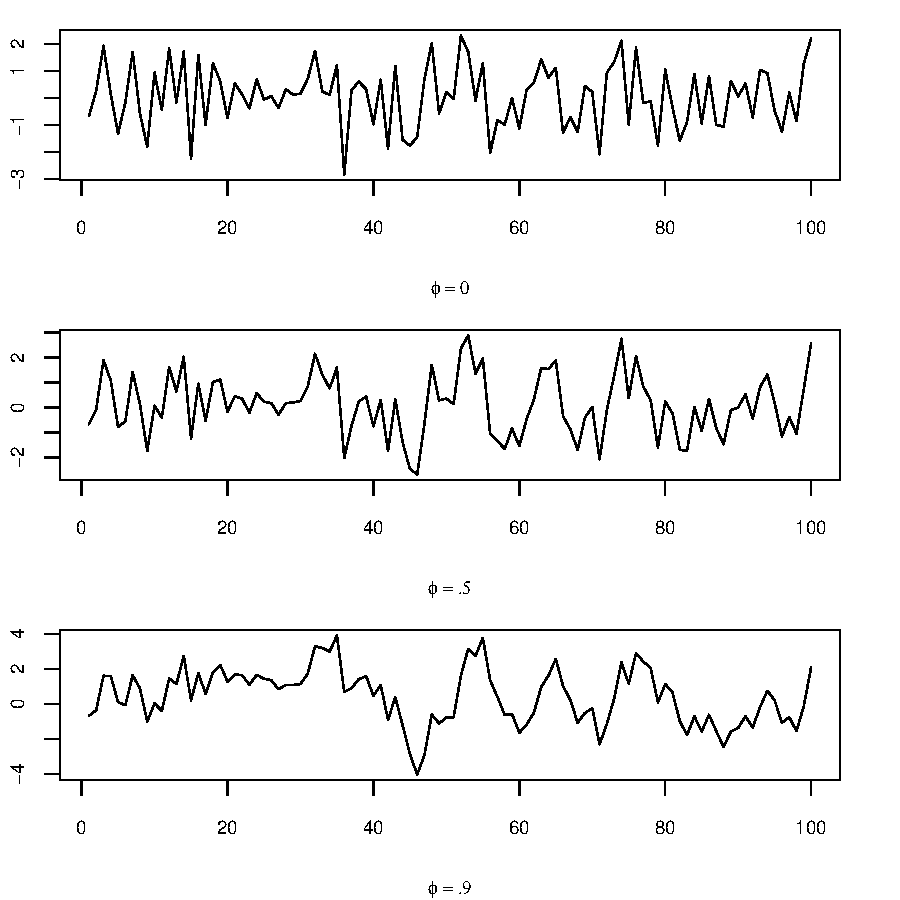
\includegraphics{p55-004}
\end{center}
\subsection{R Facilities for simulating ARMA process}
Function "simulate.forward" is a special case of capabilities provided by
the function arima.sim in package stats, as the following code verifies.
\begin{Schunk}
\begin{Sinput}
> for (specification in specifications) {
+     AR <- specification$AR
+     MA <- specification$MA
+     shift <- max(length(AR), length(MA))
+     Y <- arima.sim(model = list(order = c(length(AR), 0, length(MA)), 
+         ar = AR, ma = MA), n = T, innov = epsilon[1:T], n.start = max(shift, 
+         1), start.innov = rep(0, max(shift, 1)))
+     print(specification$Y[1:10])
+     print(Y[1:10])
+ }
\end{Sinput}
\begin{Soutput}
 [1] -0.6762810  0.2606135  1.9305498  0.1394724 -1.3271651 -0.1626523
 [7]  1.7030423 -0.5835851 -1.8031651  0.9407337
 [1] -0.6762810  0.2606135  1.9305498  0.1394724 -1.3271651 -0.1626523
 [7]  1.7030423 -0.5835851 -1.8031651  0.9407337
 [1] -0.67628102 -0.07752699  1.89178631  1.08536552 -0.78448235 -0.55489345
 [7]  1.42559560  0.12921272 -1.73855878  0.07145431
 [1] -0.67628102 -0.07752699  1.89178631  1.08536552 -0.78448235 -0.55489345
 [7]  1.42559560  0.12921272 -1.73855878  0.07145431
 [1] -0.6762810 -0.3480394  1.6173143  1.5950553  0.1083846 -0.0651061
 [7]  1.6444468  0.8964171 -0.9963898  0.0439829
 [1] -0.6762810 -0.3480394  1.6173143  1.5950553  0.1083846 -0.0651061
 [7]  1.6444468  0.8964171 -0.9963898  0.0439829
\end{Soutput}
\end{Schunk}
